%%%%%%%%%%%%%%%%%%%%%
% Documento maestro %
%%%%%%%%%%%%%%%%%%%%%
\documentclass{fime}

%%%%%%%%%%%%%%%%%%%%%%%%%%%%%%%%%%%%%%%%%%%
% Cargando paquetes y definiendo opciones %
%%%%%%%%%%%%%%%%%%%%%%%%%%%%%%%%%%%%%%%%%%%
% Aquí puedes cargar los paquetes que vas a usar. La clase
% fime ya incluye babel, inputenc, graphicx y los de la AMS.
% Cargar un paquete está a tu libertad (y responsabilidad).
\usepackage{hyperref}
\usepackage{graphicx}
\usepackage{pdflscape}
\usepackage{amsmath}
\usepackage[utf8]{inputenc}
\usepackage[numbers,sort&compress]{natbib}
\usepackage[bottom]{footmisc}
\usepackage{float}
\usepackage{footmisc}
\usepackage{adjustbox}
\usepackage{tikz}
\usepackage{url}
\usepackage{listings}
\usepackage{makecell}
\renewcommand{\cellalign}{l}
\renewcommand{\theadalign}{l}

\setlength{\footnotesep}{0.5cm}
\setlength\footnotemargin{3pt}

    \hypersetup{breaklinks=true,colorlinks=true,
        linkcolor=black,citecolor=black,urlcolor=black}

\lstset{basicstyle=\ttfamily}

%%%%%%%%%%%%%%%%%%%%%
% Definiendo campos %
%%%%%%%%%%%%%%%%%%%%%
\def\titulo{Sentiment Analysis through a chatbot}
\def\autor{Alexander Espronceda Gómez}
\def\matricula{1742000}
\def\grado{Ingeniería en Tecnología de Software}
% En caso de que el grado tenga orientación o especialidad llenar el siguiente
% campo dejando un ESPACIO INICIAL, en caso contrario, dejar vacío
\def\orientacion{}
\def\fecha{Enero 2022} % Coloca el mes con mayúscula inicial

\def\asesor{Dra. Satu Elisa Schaeffer}
\def\revisorA{Dra. Sara Elena Garza Villarreal}
\def\revisorB{Dr. Romeo Sánchez Nigenda}
% En el caso de que tu tesis sea de doctorado activa la variable cambiándola a \doctoradotrue
% y define tus otros dos revisores
\newif\ifdoctorado\doctoradofalse
\def\revisorC{Nombre del revisor C}
\def\revisorD{Nombre del revisor D}
% El visto bueno siempre va
\def\vobo{Dr. Fernando Banda Muñoz}

%%%%%%%%%%%%%%%%%%%%%%%
% Inicia el documento %
%%%%%%%%%%%%%%%%%%%%%%%
\begin{document}

\frontmatter
\pagestyle{main}

%%% Incluye PortillasM si tu tesis es de Maestría
%%% y PortillasD si es de doctorado.
% Portadas (Maestría)

\def\uanl{Universidad Autónoma de Nuevo León}
\def\fime{Facultad de Ingeniería Mecánica y Eléctrica}
\def\depg{Subdirección Académica}
\def\snnl{San Nicolás de los Garza, Nuevo León}

%%%%%%%%%%%%%%%%%%%%%%%%
% Primer portada: UANL %
%%%%%%%%%%%%%%%%%%%%%%%%
\thispagestyle{empty}

\begin{scshape}
\begin{center}
	{\Large \uanl} \\[5mm]
	{\large \fime} \\[5mm]
	{\large \depg}
	\vskip 15mm
	
\includegraphics[height=55mm]{uanl}
	\vskip 12mm
	\begin{tabular}{p{11cm}}
		\centering
		{\large \titulo}
	\end{tabular}
	\vskip 7mm
	{por}\\[7mm]
	{\large \autor}\\[7mm]
	{como requisito parcial para obtener el grado de}\\[3mm]
	\MakeUppercase{\grado}\\
	\orientacion
	\vfill
	\fecha
\end{center}
\end{scshape}

%%%%%%%%%%%%%%%%%%%%%%%%%
% Segunda portada: FIME %
%%%%%%%%%%%%%%%%%%%%%%%%%
\newpage
\thispagestyle{empty}

\begin{scshape}
\begin{center}
	{\Large \uanl} \\[5mm]
	{\large \fime} \\[5mm]
	{\large \depg}
	\vskip 16mm
	
\includegraphics[height=50mm]{fime}
	\vskip 16mm
	\begin{tabular}{p{11cm}}
		\centering
		{\large \titulo}
	\end{tabular}
	\vskip 7mm
	{por}\\[7mm]
	{\large \autor}\\[7mm]
	{como requisito parcial para obtener el grado de}\\[3mm]
	\MakeUppercase{\grado}\\
	\orientacion
	\vfill
	\fecha
\end{center}
\end{scshape}

%%%%%%%%%%%%%%%%%%%%%%%%%%%%%
% Carta del comité de tesis %
%%%%%%%%%%%%%%%%%%%%%%%%%%%%%
\newpage
\thispagestyle{empty}
\enlargethispage{5mm}

\begin{center}
{\bf \large \uanl} \\
{\bf \fime} \\
{\bf \depg}
\end{center}
\vskip 4mm

Los miembros del Comité de Tesis recomendamos que la Tesis \guillemotleft\titulo\guillemotright, realizada por el alumno \autor, con número de matrícula \matricula, sea aceptada para su defensa como requisito parcial para obtener el grado de \grado\orientacion.
\ifdoctorado{\vskip 10mm}\else{\vskip 8mm}\fi

\begin{center}
El Comité de Tesis\\
\ifdoctorado{\vskip 15mm}\else{\vskip 25mm}\fi

\ifdoctorado{%%%
\begin{tabular}{p{37mm}p{21mm}p{12mm}p{21mm}p{37mm}}
	\cline{2-4}
	& \multicolumn{3}{c}{\asesor} & \\
	& \multicolumn{3}{c}{Asesora}  & \\[15mm]
	\cline{1-2} \cline{4-5}
	\multicolumn{2}{c}{\revisorA} & & \multicolumn{2}{c}{\revisorB} \\
	\multicolumn{2}{c}{Revisora}   & & \multicolumn{2}{c}{Revisor}   \\[17mm]
	\cline{1-2} \cline{4-5}
	\multicolumn{2}{c}{\revisorC} & & \multicolumn{2}{c}{\revisorD} \\
	\multicolumn{2}{c}{Revisor}   & & \multicolumn{2}{c}{Revisor}   \\[2mm]
	& \multicolumn{3}{c}{Vo. Bo.} & \\[14mm]
	\cline{2-4}
	& \multicolumn{3}{c}{\vobo}   & \\
	& \multicolumn{3}{c}{\depg}   & \\ &&&&
\end{tabular}
}\else{%%%
\begin{tabular}{p{37mm}p{21mm}p{12mm}p{21mm}p{37mm}}
	\cline{2-4}
	& \multicolumn{3}{c}{\asesor} & \\
	& \multicolumn{3}{c}{Asesora}  & \\[19mm]
	\cline{1-2} \cline{4-5}
	\multicolumn{2}{c}{\revisorA} & & \multicolumn{2}{c}{\revisorB} \\
	\multicolumn{2}{c}{Revisora}   & & \multicolumn{2}{c}{Revisor}   \\[2mm]
	& \multicolumn{3}{c}{Vo. Bo.} & \\[17mm]
	\cline{2-4}
	& \multicolumn{3}{c}{\vobo}   & \\
	& \multicolumn{3}{c}{\depg}   & \\ &&&&
\end{tabular}
}\fi%%%

\vfill

\snnl, \MakeLowercase{\fecha}

\end{center}

%%%% Dedicatoria

\thispagestyle{empty}
\vspace*{17mm}

\begin{flushright}
\begin{itshape}

Aquí puedes poner tu dedicatoria\\
si es que tienes una.\bigskip\bigskip

Si no tienes una, puedes borrar\\
la línea \verb+% Dedicatoria

\thispagestyle{empty}
\vspace*{17mm}

\begin{flushright}
\begin{itshape}

Aquí puedes poner tu dedicatoria\\
si es que tienes una.\bigskip\bigskip

Si no tienes una, puedes borrar\\
la línea \verb+% Dedicatoria

\thispagestyle{empty}
\vspace*{17mm}

\begin{flushright}
\begin{itshape}

Aquí puedes poner tu dedicatoria\\
si es que tienes una.\bigskip\bigskip

Si no tienes una, puedes borrar\\
la línea \verb+\include{Dedicatoria}+ en el\\
archivo \texttt{MiTesis.tex} pues no es obligatoria.

\end{itshape}
\end{flushright}

+ en el\\
archivo \texttt{MiTesis.tex} pues no es obligatoria.

\end{itshape}
\end{flushright}

+ en el\\
archivo \texttt{MiTesis.tex} pues no es obligatoria.

\end{itshape}
\end{flushright}



\tableofcontents
\listoffigures
\listoftables

%Agradecimientos

\chapter{Agradecimientos}
\markboth{Agradecimientos}{}

--------(WORK IN PROGRESS)--------
%Resumen

\chapter{Resumen}
\markboth{Resumen}{}

{\setlength{\leftskip}{10mm}
\setlength{\parindent}{-10mm}

\autor.

Candidato para obtener el grado de \grado\orientacion.

\uanl.

\fime.

Título del estudio: \textsc{\titulo}.

\noindent Número de páginas: \pageref*{lastpage}.}

%%% Comienza a llenar aquí
\paragraph{Objetivos y Método de Estudio:}
En esta tesis se propone generar software de uso libre que interprete el texto introducido por un usuario y determine su estado de ánimo, con el propósito de usarse en conjunto con otro software o algoritmos con enfoque en datos conversacionales.

El método de estudio utilizado hará un análisis comprensivo de las redes neuronales y aprendizaje máquina supervisado, así como también de reconocimiento de patrones y recopilación de datos que nos dé comprensión moderada de algo tan voluble y a veces impredecible como lo es la mente humana.
\newpage
\paragraph{Contribuciones y Conclusiones:}
El algoritmo de entrenamiento utiliza un conjunto de datos específico para predecir, dentro de lo posible, qué está sintiendo una persona al momento de escribir alguna oración o frase. El algoritmo resultante es open-source por lo que cualquier persona puede añadir o quitar módulos según se requiera, y utilizarlo en otros proyectos.

La conclusión de esta tesis es que es posible que un algoritmo de Red Neuronal Recurrente reconozca los patrones de una frase usando código open-source, pero se tiene que tener un conjunto de datos limpio, bien distribuido y que incluya palabras que sean difíciles de clasificar erróneamente.

\bigskip\noindent\begin{tabular}{lc}
\vspace*{-2mm}\hspace*{-2mm}Firma de la asesora: & \\
\cline{2-2} & \hspace*{1em}\asesor\hspace*{1em}
\end{tabular}




\mainmatter
\pagestyle{fime}

%%% Haz un documento para cada capítulo
\chapter{Introduction}
Human beings are social beings, this is widely known. To survive, we must band together and communicate with each other, bonding in the process. This is thanks to a neural process called \textbf{empathy}, which is defined as a three-part process that happens in our brains \citep{rf1}. That roughly happens like this:
\begin{itemize}
	\item Emotional simulation centered in the limbic system, which makes us mirror the emotional elements we're watching.
	\item Processing the perspective in the prefrontal and temporal cortex.
	\item Assessing the course of action to take, either showing compassion or doing something else. This is allegedly based in the obitofrontal cortex, as well as several other parts of the brain.
\end{itemize}
This is clearly what we consider a normally human-only behavior, but there's been studies that indicate that apes, dogs and rodents have been observed to take action at the presence of distress signals, either from humans or other members of their own species \citep{rf2}.
If this is true, theoretically, we could teach a machine learning algorithm to process signals of distress and react accordingly.

\section{Motivation}
At first, I wanted to create an algorithm that could serve as a makeshift therapy chatbot that people could use when they were confused about their own feelings, but as time has passed, a lot of things have happened in my life regarding people with close-to-none empathy.
This project could prove especially useful towards people who have trouble discerning when to console someone or having an idea of how other people or even themselves feel, such as the case of people with Asperger's Syndrome or other forms of high-functioning autism.
To this end, I've decided to work on this project.

\section{Hypothesis}
Empathy consists in a pattern of neurochemical reactions triggered by different situations. Machine learning could learn to identify these patterns without them being processed biologically.

\section{Objectives}
In this section, I will establish the objectives I would like to touch upon in this paper.

\subsection{General Objectives}
The objective of this project is to determine how the user's feeling according to the words in the input. This will be achieved thanks to the technology present in machine learning algorithms and an extensive amount of datasets.

\subsection{Specific Objectives}
\begin{itemize}
	\item Generating an algorithm capable of detecting key words related to the user's mood.
	\item Predicting successfully the user's mood according to their input.
\end{itemize}

\section{Structure}
---Work in progress---
\clearpage
\chapter{Introduction}
Human beings are social beings, this is widely known. To survive, we must band together and communicate with each other, bonding in the process. This is thanks to a neural process called \textbf{empathy}, which is defined as a three-part process that happens in our brains \citep{rf1}. That roughly happens like this:
\begin{itemize}
	\item Emotional simulation centered in the limbic system, which makes us mirror the emotional elements we're watching.
	\item Processing the perspective in the prefrontal and temporal cortex.
	\item Assessing the course of action to take, either showing compassion or doing something else. This is allegedly based in the obitofrontal cortex, as well as several other parts of the brain.
\end{itemize}
This is clearly what we consider a normally human-only behavior, but there's been studies that indicate that apes, dogs and rodents have been observed to take action at the presence of distress signals, either from humans or other members of their own species \citep{rf2}.
If this is true, theoretically, we could teach a machine learning algorithm to process signals of distress and react accordingly.

\section{Motivation}
At first, I wanted to create an algorithm that could serve as a makeshift therapy chatbot that people could use when they were confused about their own feelings, but as time has passed, a lot of things have happened in my life regarding people with close-to-none empathy.
This project could prove especially useful towards people who have trouble discerning when to console someone or having an idea of how other people or even themselves feel, such as the case of people with Asperger's Syndrome or other forms of high-functioning autism.
To this end, I've decided to work on this project.

\section{Hypothesis}
Empathy consists in a pattern of neurochemical reactions triggered by different situations. Machine learning could learn to identify these patterns without them being processed biologically.

\section{Objectives}
In this section, I will establish the objectives I would like to touch upon in this paper.

\subsection{General Objectives}
The objective of this project is to determine how the user's feeling according to the words in the input. This will be achieved thanks to the technology present in machine learning algorithms and an extensive amount of datasets.

\subsection{Specific Objectives}
\begin{itemize}
	\item Generating an algorithm capable of detecting key words related to the user's mood.
	\item Predicting successfully the user's mood according to their input.
\end{itemize}

\section{Structure}
---Work in progress---
\clearpage
\chapter{Project Development}

\section{Datasets}
There are several datasets on the internet, but none of them have the amount of sheer volume and actually useful data that is required for this task. The closest available was used, however, and it brought relatively acceptable levels of accuracy \citep{rf7}.
This dataset, paired with NLTK processing, stopwords and truncating words and verbs commonly used in the English language, was able to pinpoint if the user had a positive, neutral or a negative feeling in their input about 40\% of the time, approximately.
This is not really a good number for such a small amount of labels, but it's an improvement nonetheless. Previous versions with different approaches, combination of layers and datasets had less than 20\% of accuracy.
\pagebreak

\section{Algorithm Used}
A standard LSTM algorithm was used with a softmax activation end layer. After much, much testing \textit{rmsprop} was chosen as the optimizer because of its slightly better results.
\begin{figure}[!h]
	\centering
	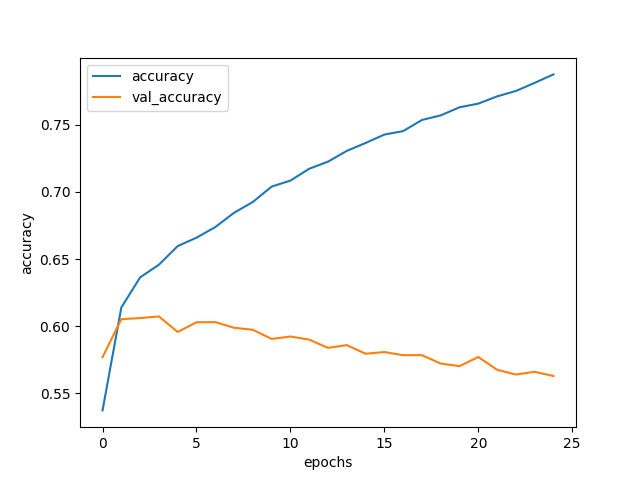
\includegraphics[scale=0.6]{Accuracy 2021-05}
	\caption{Accuracy Graph of the Algorithm Training}
	\label{fig:accuracy}
	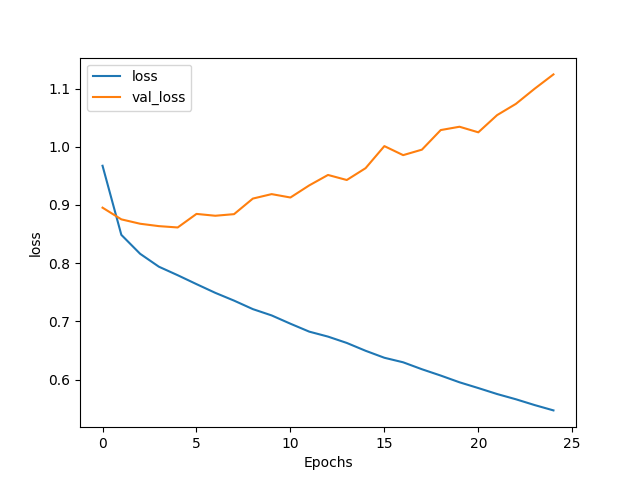
\includegraphics[scale=0.6]{Loss 2021-05}
	\caption{Loss Graph of the Algorithm Training}
	\label{fig:loss}
\end{figure}
\begin{figure}[!h]
	\centering
	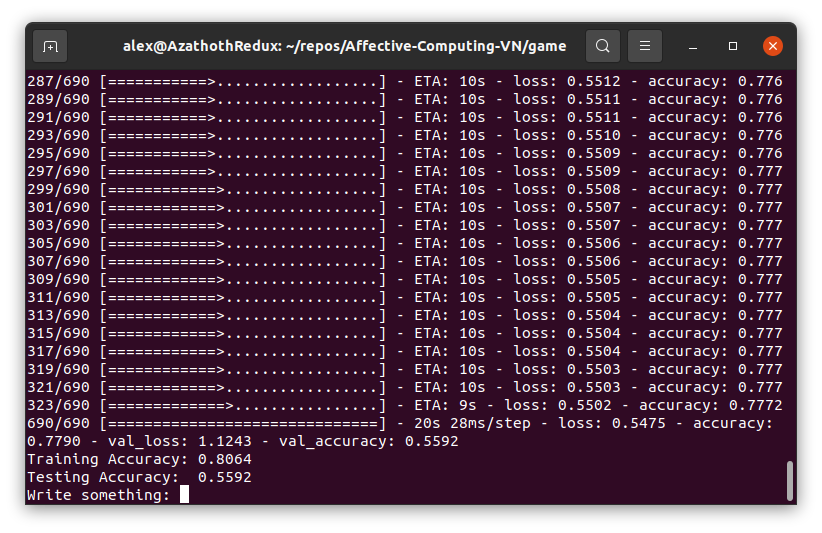
\includegraphics[scale=0.4]{Test 2021-05}
	\caption{Debugging of the Trained Model}
	\label{fig:test}
\end{figure}
\pagebreak

\section{Interface}
Originally, \textit{Ren'py}\footnote{An open-source Python framework focused mostly in the development of visual novels and other videogame formats. \url{https://www.renpy.org/}} was the chosen framework for this project's interface to work with, but -- unfortunately for the proposed usage -- it only works with Python 2.7, which makes it incompatible with TensorFlow 2.0. Making a bridge between Python 2 and 3 would inevitably generate more issues that would take more time to solve, so it was scrapped in favor of the \textit{pygame} library.
\begin{figure}[!h]
	\centering
	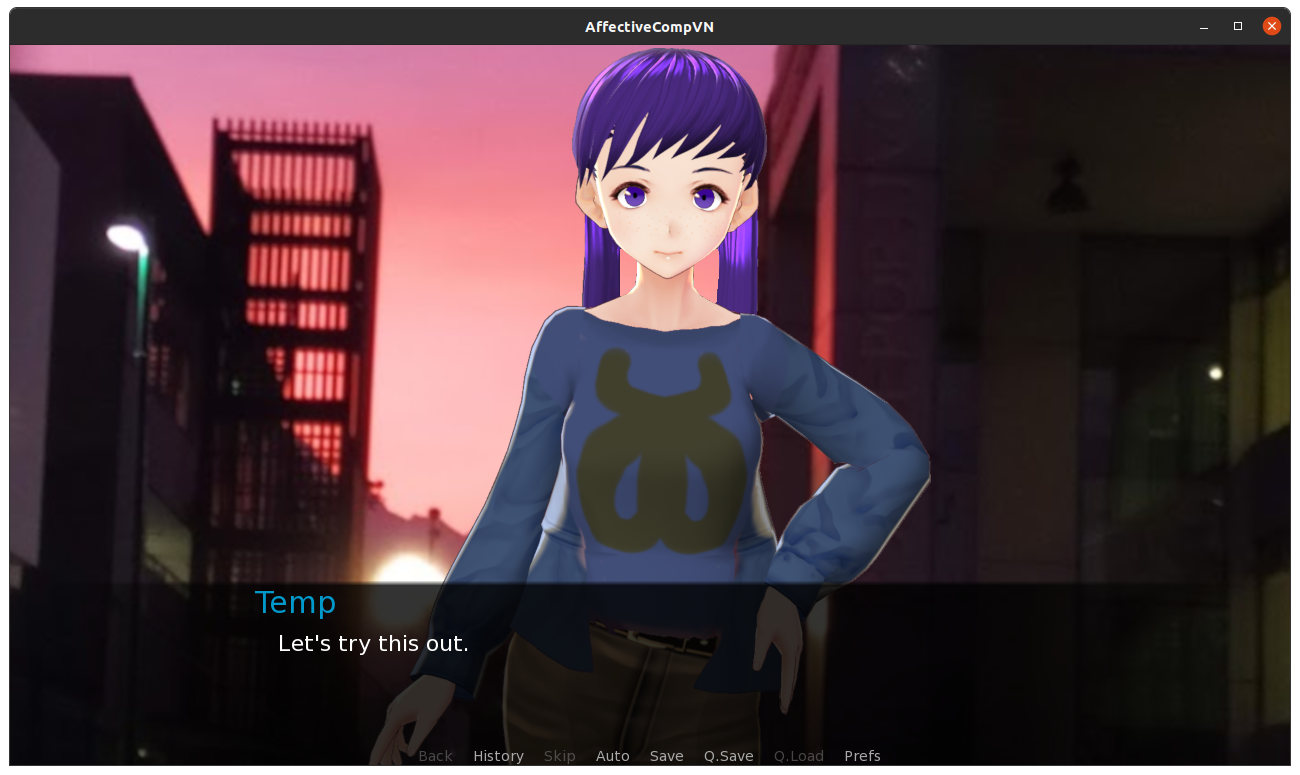
\includegraphics[scale=0.3]{Ren'py}
	\caption{First version of the interface using Ren'py}
	\label{fig:renpy_test_1}
\end{figure}
\begin{figure}[!h]
	\centering
	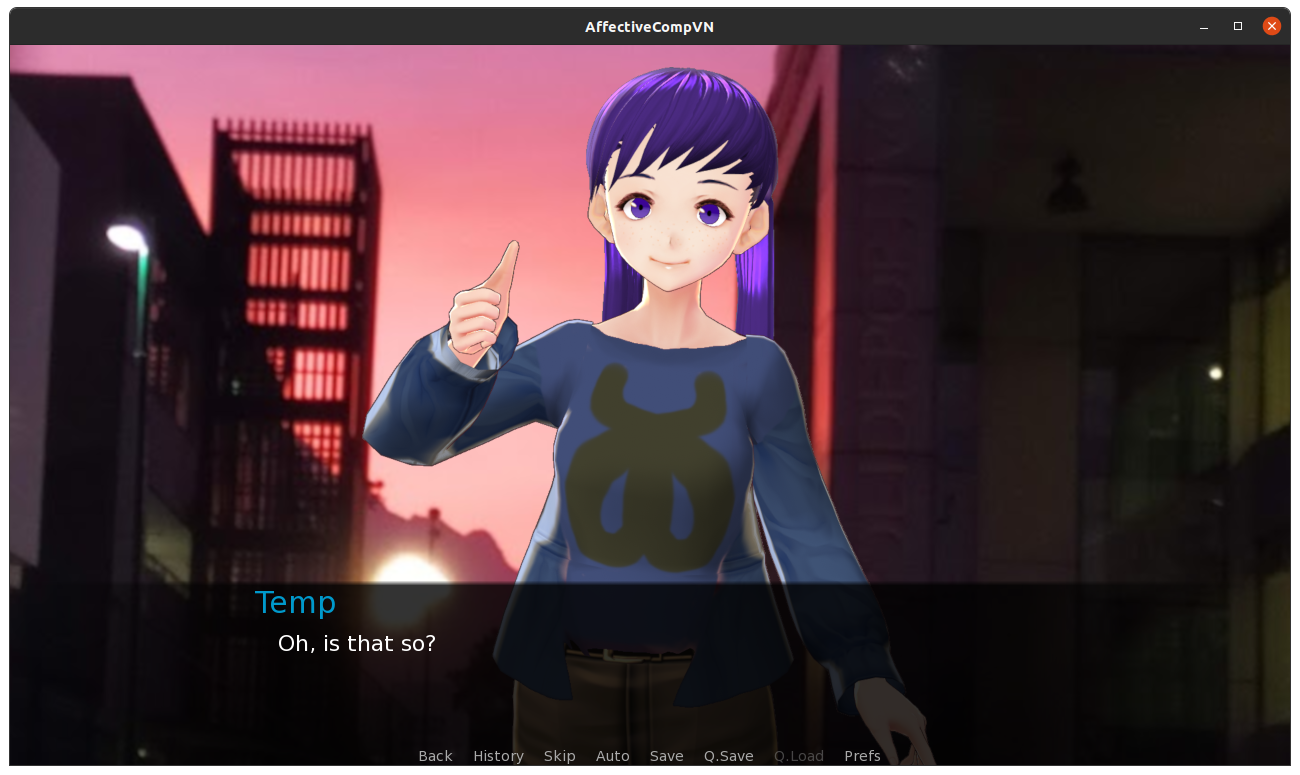
\includegraphics[scale=0.3]{Ren'py_2}
	\caption{Reacting positively to an user's feedback}
	\label{fig:renpy_test_2}
\end{figure}
As for the character that's being used, it's also gone through some changes. Originally the idea was to make a low-poly character render to work with, but since 3D modeling-from-scratch skills exceed the scope of this paper, an alternative software was selected instead. Namely \textit{VRoid}.



\chapter{Project Development}

\section{Datasets}
There are several datasets on the internet, but none of them have the amount of sheer volume and actually useful data that is required for this task. The closest available was used, however, and it brought relatively acceptable levels of accuracy \citep{rf7}.
This dataset, paired with NLTK processing, stopwords and truncating words and verbs commonly used in the English language, was able to pinpoint if the input had a positive, neutral or a negative feeling about 40\% of the time, approximately.
This is not really a good number for such a small amount of labels, but it's an improvement nonetheless. Previous versions with different approaches, combination of layers and datasets had less than 20\% of accuracy.
\pagebreak

\subsection{Pre-filtering}
Since the dataset that was chosen was imported straight from Twitter with little to no filtering, some cleanup had to be done to ensure peak performance.
The first problem was the punctuation marks, which were easy to filter out. The issues came after this with the so-called stopwords, which are words that do not really contribute to the overall meaning of the text. Luckily, NLTK\footnote{Natural Language Toolkit, tool used specifically for these case scenarios. \url{https://www.nltk.org/}} has its own repository of these words, so it was implemented. There was also an issue where verbs in different tenses were evaluated very differently, so a  stemmer was implemented, which truncated words to its most basic features (aptly named stems) and prevented the loss to keep rising that much between epochs.
\pagebreak
\begin{figure}[!h]
	\centering
	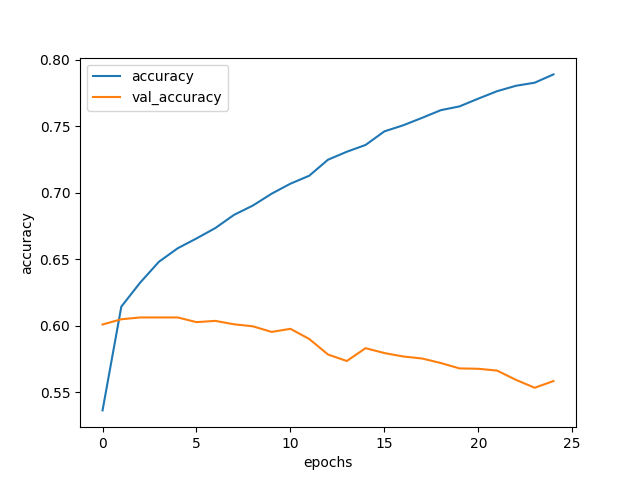
\includegraphics[scale=0.6]{Accuracy 2020-05}
	\caption{Accuracy Graph of the Algorithm Training on May 2020, with no NLTK stemming}
	\label{fig:accuracy2020_nofilter}
	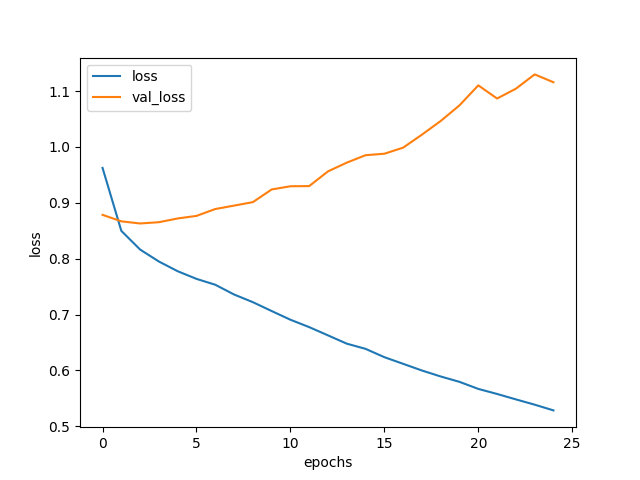
\includegraphics[scale=0.6]{Loss 2020-05}
	\caption{Loss Graph of the Algorithm Training on May 2020, with no NLTK stemming}
	\label{fig:loss2020_nofilter}
\end{figure}

\subsection{Filtering}
The dataset itself has several different sentiment labels to analyze, the ones being considered in the scope of this paper are:
\begin{itemize}
	\item Sadness
	\item Neutral
	\item Happiness
	\item Fun
	\item Worry
	\item Boredom
\end{itemize}
But since they are not evenly distributed, leaving them as-is led to very inaccurate results, so a generalistic approach was opted for, classifying the end results in ``Good'', ``Neutral'' and ``Bad'' depending on the overall wellness percieved from the input.
This final filter works only with the training data, and works as follows:
\begin{itemize}
	\item Sadness and Worry are in the ``Bad'' category.
	\item Neutral and Boredom are in the ``Neutral'' category.
	\item Happiness and Fun are in the ``Good'' category
\end{itemize}
Using a more complicated classification process would take an even amount of data in every category. Which, at the time of writing, no dataset readily available has.

\section{Algorithm Used}
A bidirectional LSTM algorithm was used with a softmax activation end layer. After much, much testing \textit{rmsprop} was chosen as the optimizer because of its slightly better results overall.
The internal lexicon is limited to 5000 items, and the maximum length of any given phrase after filtering is 30 characters.
The training consists in 25 epochs on 75\% of the dataset on a random arbitrary order, using the remaining 25\% for validation instead.
\begin{figure}[!h]
	\centering
	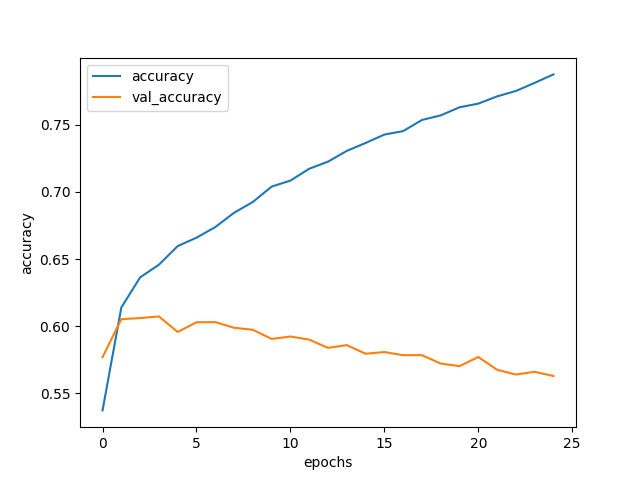
\includegraphics[scale=0.6]{Accuracy 2021-05}
	\caption{Accuracy Graph of the Algorithm Training on May 2021}
	\label{fig:accuracy2021}
	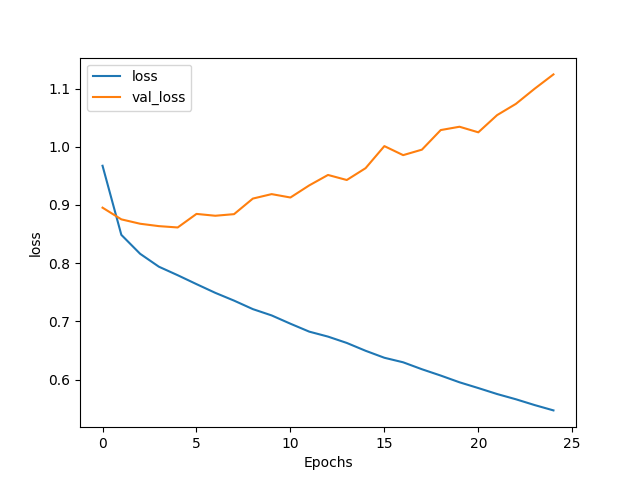
\includegraphics[scale=0.6]{Loss 2021-05}
	\caption{Loss Graph of the Algorithm Training on May 2021}
	\label{fig:loss2021}
\end{figure}
\begin{figure}[!h]
	\centering
	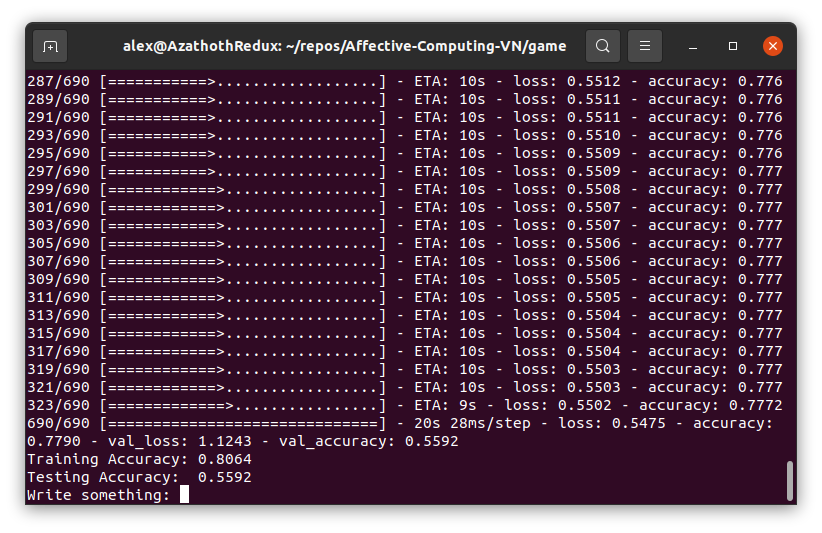
\includegraphics[scale=0.4]{Test 2021-05}
	\caption{Debugging of the Trained Model}
	\label{fig:test}
\end{figure}
\pagebreak

\section{Interface}
Originally, \textit{Ren'py}\footnote{An open-source Python framework focused mostly in the development of visual novels and other videogame formats. \url{https://www.renpy.org/}} was the chosen framework for this project's interface to work with, but -- unfortunately for the proposed usage -- it only works with Python 2.7, which makes it incompatible with TensorFlow 2.0. Making a bridge between Python 2 and 3 would inevitably generate more issues that would take more time to solve, so it was scrapped in favor of the \textit{pygame} library.
\pagebreak

\begin{figure}[!h]
	\centering
	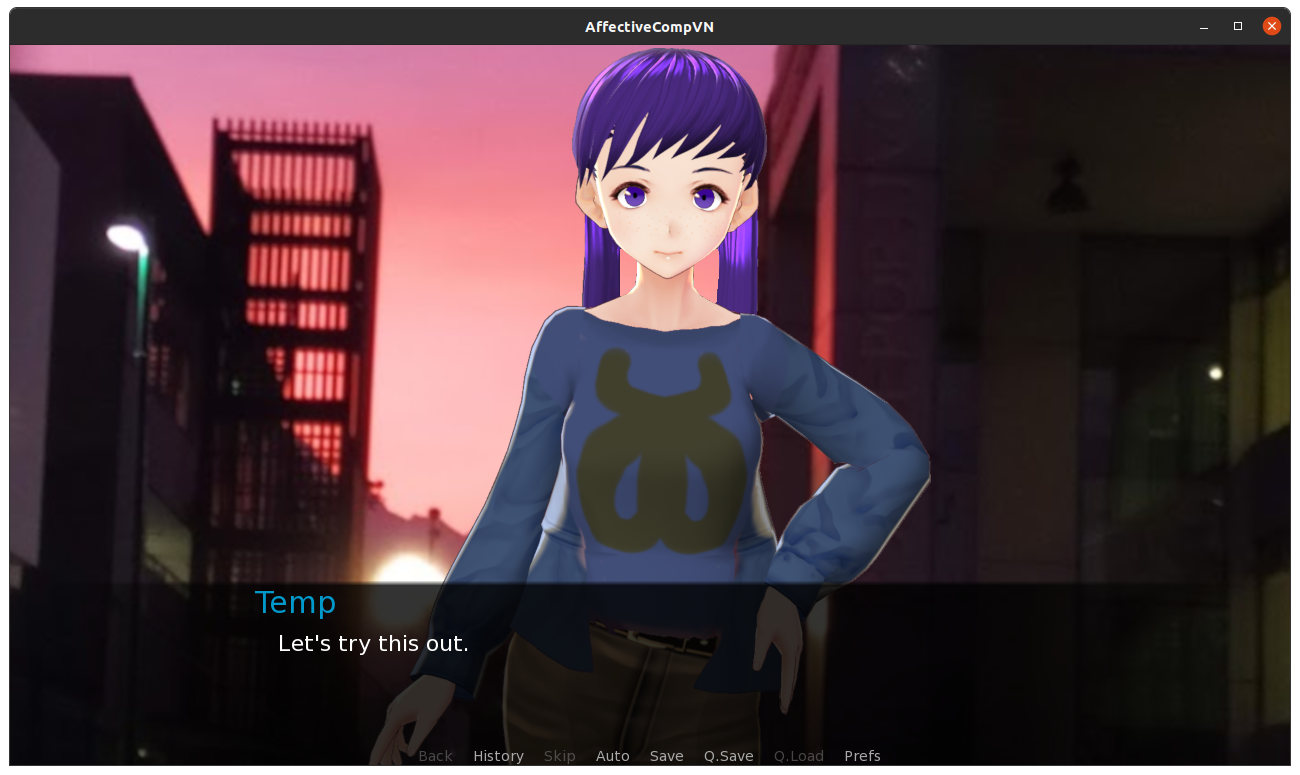
\includegraphics[scale=0.3]{Ren'py}
	\caption{First version of the interface using Ren'py}
	\label{fig:renpy_test_1}
\end{figure}
\begin{figure}[!h]
	\centering
	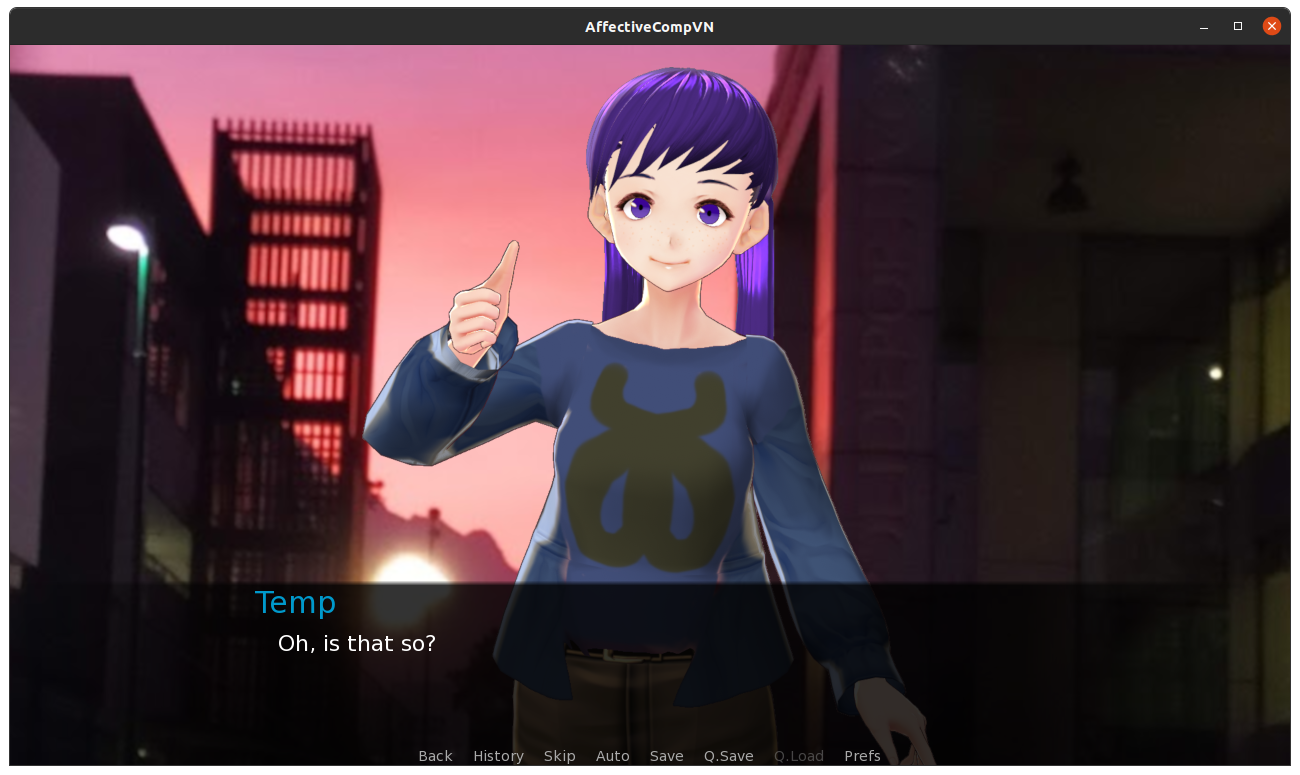
\includegraphics[scale=0.3]{Ren'py_2}
	\caption{Reacting positively to text in the ``Good'' category}
	\label{fig:renpy_test_2}
\end{figure}

The current interface is a hybrid between a Pygame screen, where the assistant appears to react to the input, and the console, where a person can input text to be analyzed.
\pagebreak

\subsection{Assistant}
As for the character that is being used, it also has gone through some changes. Originally the idea was to make a low-poly character render to work with, but since 3D modeling-from-scratch skills exceed the scope of this paper, an alternative software was selected instead. Namely \textit{VRoid}.\\
The main purpose for this assistant is to make people feel like it is her that they are talking to and not to some faceless machine, while also making it easier to the eyes. A more realistic, less animated style could have been used, but a friendly, less prone to uncanny valley approach to the design was opted for with this in mind.
\begin{figure}[!ht]
	\centering
	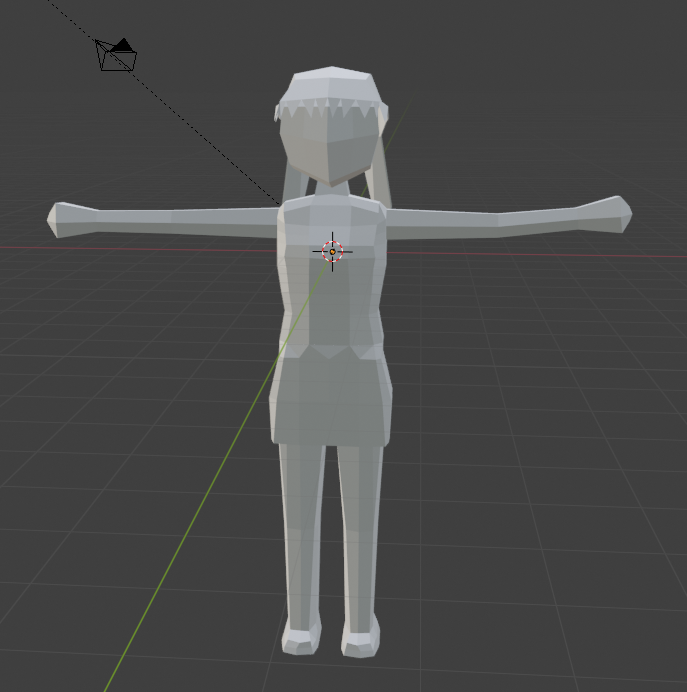
\includegraphics[scale=.5]{Assistant_1}
	\caption{First attempt at 3D modeling an assistant.}
	\label{fig:assistant1}
\end{figure}
\begin{figure}[!ht]
	\centering
	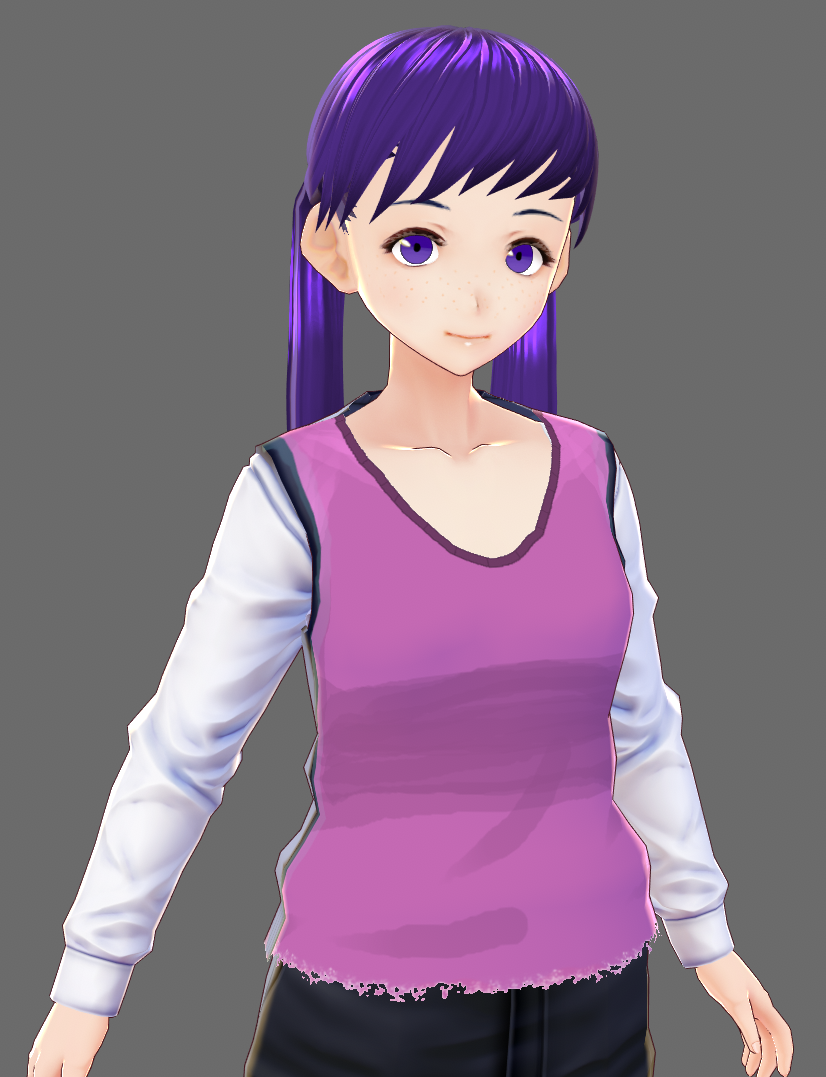
\includegraphics[scale=.25]{Assistant_2}
	\caption{Assistant Ver. 2, now using VRoid.}
	\label{fig:assistant2}
\end{figure}
\begin{figure}[!ht]
	\centering
	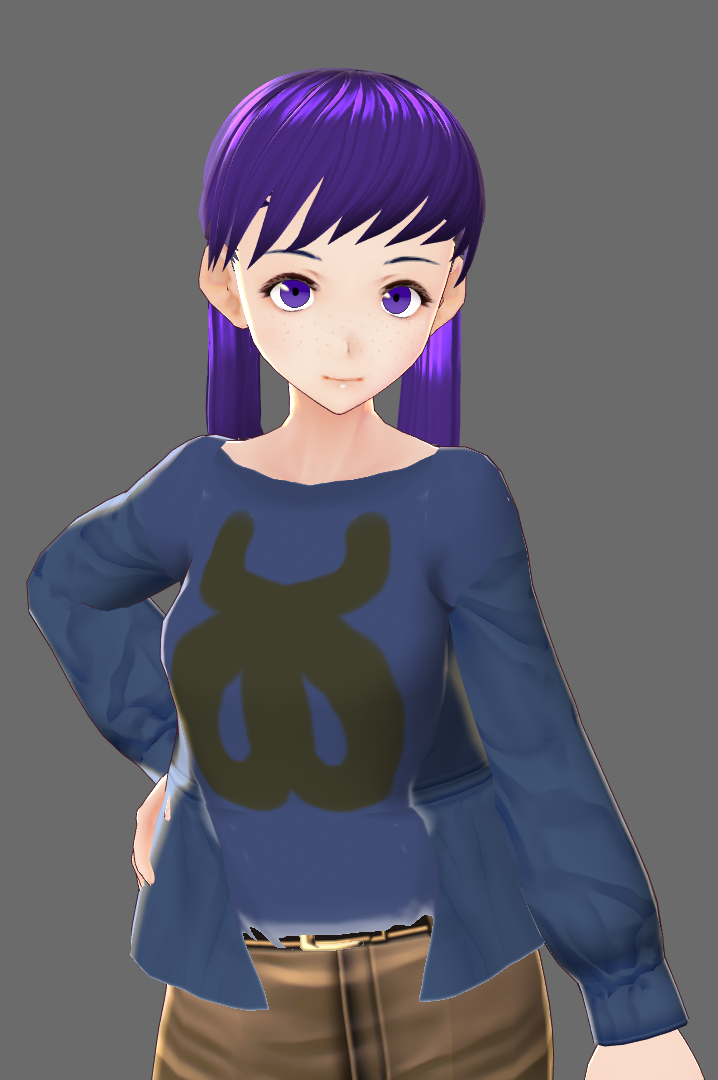
\includegraphics[scale=.25]{Assistant_3}
	\caption{Assistant Ver. 3, the current design.}
	\label{fig:assistant3}
\end{figure}



\chapter{Data Experiments}
\label{ch5}
In this chapter, the parts that compose this project as well as their context are shown. Also, some experiments are demonstrated for comparison with different parameters that could affect this thesis' project's overall accuracy.

\section{Inputs and Outputs}
In previous chapters, it has been specified that this algorithm takes an text input and, according to its contents, a message is shown as an output. The breakdown is as follows.
\subsection{Inputs}
The input that is given is cleaned up and tokenized -- as shown in \nameref{ch4} --, this is then added to an internal corpus that has weights set for every word in it, effectively working as scores. Every word has a different score in every label, whether it is positive or negative. This score is added up and the highest final score will be the one that the algorithm will detect as the most probable for the text input. However, this has its caveats, small sentences are more likely to be miscategorized because one word can have different applications in the scope of this project, for a more accurate analysis a longer sentence must be written.
\subsection{Outputs}
Depending on the final score, the algorithm will choose a random sentence related to the detected sentiment, this is, as of the time of writing, very rudimentary, but the fact that it is built in Python this can be a building block for a more robust, context-conscious, reply system.
In the training module, however, four extra values are part of the output as well: \texttt{Loss}, \texttt{Val\_loss}, \texttt{Accuracy} and \texttt{Val\_accuracy}.
These values are standard in every Neural Network algorithm to observe how poorly the evaluation does within the training dataset, and what the accuracy percentage is, respectively.
The \texttt{Val\_} counterparts of these values are the same, but applied to the validation dataset.

\section{Experiments}
In this section, various experiments of this project are shown with varying training data and parameters with the respective accuracy and loss graphs.
The purpose of these experiments is to determine if the parameters chosen for this project are optimal and, if not, correct them and know the reason behind the improvement.
The parameters that could potentially have a great impact on the output of the classification -- and therefore are the best to experiment with -- are the following:
\begin{itemize}
	\item Used datasets: This could influentiate the amount of words in the corpus and have a big impact on how some words are percieved
	\item Training epochs: How many loops does the algorithm go through before being considered fully trained, if this number is too high it could result in \textit{overfitting}, which is, in casual terms, the Neural Network equivalent of overthinking.
	\item Units in the LSTM layer: This unit system, albeit small in the overall scale of things, could make-or-break the algorithm if not tuned correctly.
	\item Categorized sentiments: Reducing the scope of the project could potentially benefit the overall accuracy of the remaining sentiments.
\end{itemize}
The amount of improvement with each experiment is shown with loss and accuracy graphs, which are evaluated every epoch the algorithm is trained. Lower loss and higher accuracy are preferred.
\subsection{Experiment 1: Base Experiment}
\label{exp1}
In this experiment, we look at the base version of this thesis' project.
\begin{table}[!th]
	\caption{Experiment 1's defining characteristics.}
	\vspace{0.5cm}
	\centering
	\begin{tabular}[t]{|l|l|}
	\hline
		Datasets Used & 2: \citet{d1} and \citet{d2}
	\\ \hline
		Epochs & 10
	\\ \hline
		LSTM Layer & 32 units
	\\ \hline
		Categorized Sentiments as ``Bad'' & ``Sadness'', ``Worry'', and ``Fear''.
	\\ \hline	
		 Categorized Sentiments as ``Neutral'' & ``Neutral'' and ``Boredom''.
	\\ \hline	
		Categorized Sentiments as ``Good'' & ``Happiness'', ``Fun'', ``Joy'', and ``Love''.
	\\ \hline
	\end{tabular}
\end{table}

\begin{figure}[!h]
	\centering
	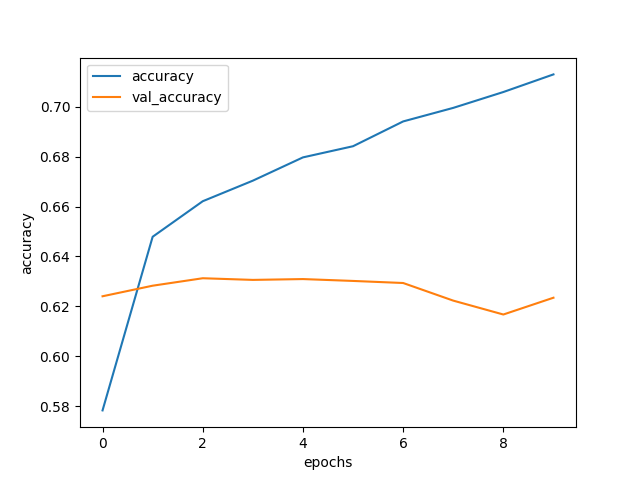
\includegraphics[scale=0.8]{Accuracy_Exp1}
	\caption{Accuracy Graph of Experiment 1}
	\label{fig:accuracy_exp1}
	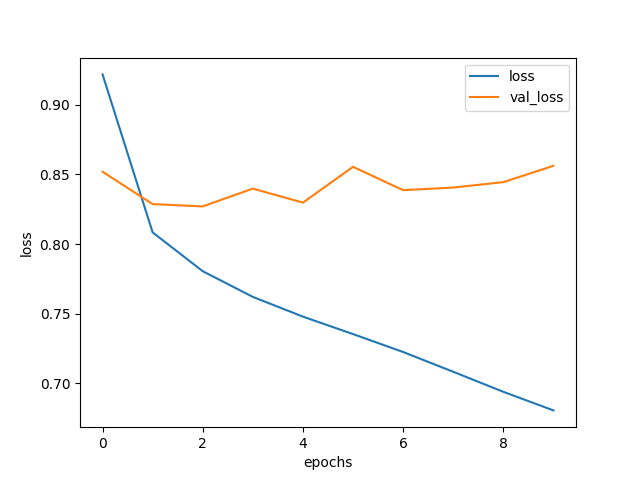
\includegraphics[scale=0.8]{Loss_Exp1}
	\caption{Loss Graph of Experiment 1}
	\label{fig:loss_exp1}
\end{figure}
\pagebreak

\subsection{Experiment 2: More Datasets With Reduced Data Scope}
\label{exp2}
This experiment takes sentences from one more dataset and 3 less categorized sentiments: ``Fear'', ``Joy'', and ``Love''.
\begin{table}[!th]
	\caption{Experiment 2's defining characteristics.}
	\vspace{0.5cm}
	\centering
	\begin{tabular}[t]{|l|l|}
	\hline
		Datasets Used & \makecell{3: \citet{d1}, \citet{d2} and\\ \citet{d3}}
	\\ \hline
		Epochs & 10
	\\ \hline
		LSTM Layer & 32 units
	\\ \hline
		Categorized Sentiments as ``Bad'' & ``Sadness'', and ``Worry''.
	\\ \hline	
		 Categorized Sentiments as ``Neutral'' & ``Neutral'' and ``Boredom''.
	\\ \hline	
		Categorized Sentiments as ``Good'' & ``Happiness'', and ``Fun''.
	\\ \hline
	\end{tabular}
\end{table}

\begin{figure}[!h]
	\centering
	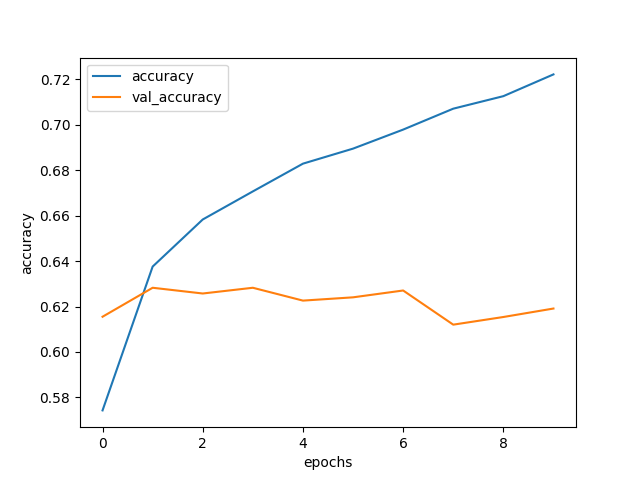
\includegraphics[scale=0.8]{Accuracy_Exp2}
	\caption{Accuracy Graph of Experiment 2}
	\label{fig:accuracy_exp2}
	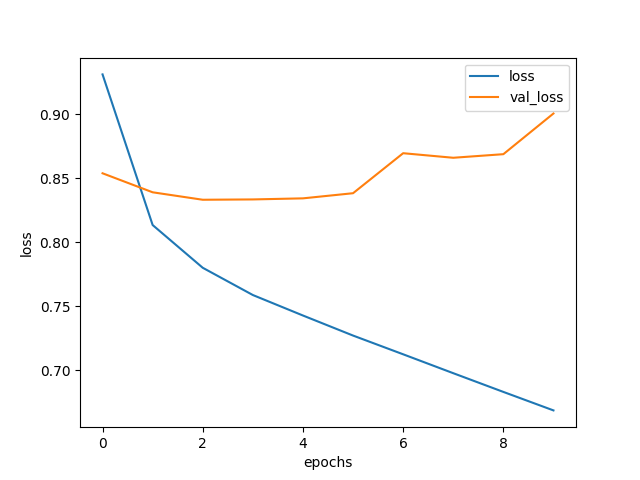
\includegraphics[scale=0.8]{Loss_Exp2}
	\caption{Loss Graph of Experiment 2}
	\label{fig:loss_exp2}
\end{figure}
\pagebreak

\subsection{Experiment 3: Augmented LSTM Units}
\label{exp3}
Largely the same as Experiment 2, but the LSTM has more units to work with.
\begin{table}[!th]
	\caption{Experiment 3's defining characteristics.}
	\vspace{0.5cm}
	\centering
	\begin{tabular}[t]{|l|l|}
	\hline
		Datasets Used & \makecell{3: \citet{d1}, \citet{d2} and\\ \citet{d3}}
	\\ \hline
		Epochs & 10
	\\ \hline
		LSTM Layer & 64 units
	\\ \hline
		Categorized Sentiments as ``Bad'' & ``Sadness'', and ``Worry''.
	\\ \hline	
		 Categorized Sentiments as ``Neutral'' & ``Neutral'' and ``Boredom''.
	\\ \hline	
		Categorized Sentiments as ``Good'' & ``Happiness'', and ``Fun''.
	\\ \hline
	\end{tabular}
\end{table}

\begin{figure}[!h]
	\centering
	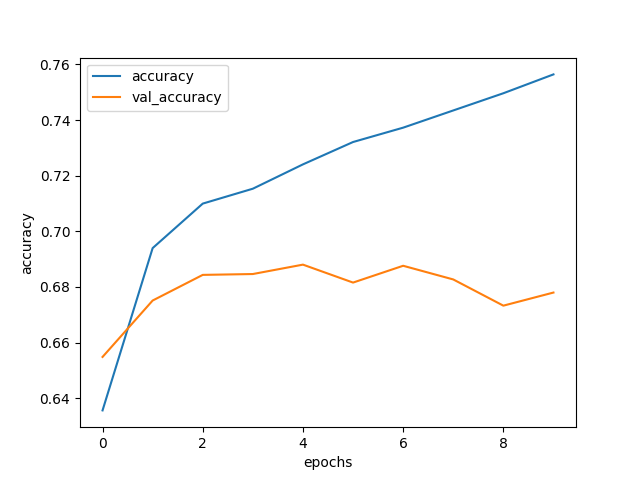
\includegraphics[scale=0.8]{Accuracy_Exp3}
	\caption{Accuracy Graph of Experiment 3}
	\label{fig:accuracy_exp3}
	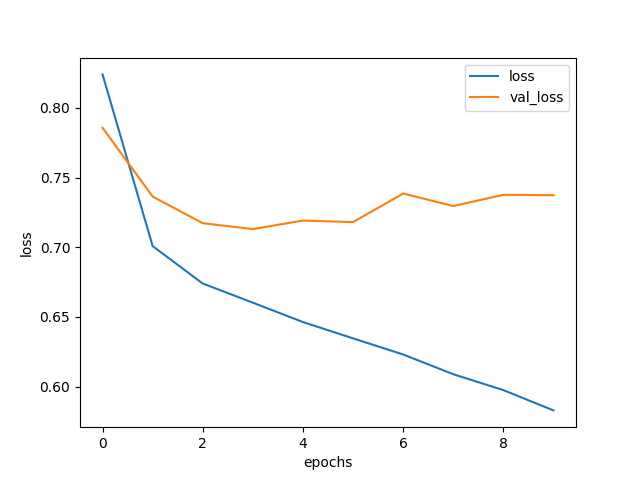
\includegraphics[scale=0.8]{Loss_Exp3}
	\caption{Loss Graph of Experiment 3}
	\label{fig:loss_exp3}
\end{figure}
\pagebreak

\subsection{Experiment 4: Augmented Datasets Without Reduced Data Scope}
\label{exp4}
A mix between Experiment 1 and 2. Three datasets with the full sentiment categorization and LSTM with 32 units.
\begin{table}[!h]
	\caption{Experiment 4's defining characteristics.}
	\vspace{0.5cm}
	\centering
	\begin{tabular}[t]{|l|l|}
	\hline
		Datasets Used & \makecell{3: \citet{d1}, \citet{d2} and\\ \citet{d3}}
	\\ \hline
		Epochs & 10
	\\ \hline
		LSTM Layer & 32 units
	\\ \hline
		Categorized Sentiments as ``Bad'' & ``Sadness'', ``Worry'', and ``Fear''.
	\\ \hline	
		 Categorized Sentiments as ``Neutral'' & ``Neutral'' and ``Boredom''.
	\\ \hline	
		Categorized Sentiments as ``Good'' & ``Happiness'', ``Fun'', ``Joy'', and ``Love''.
	\\ \hline
	\end{tabular}
\end{table}

\begin{figure}[!h]
	\centering
	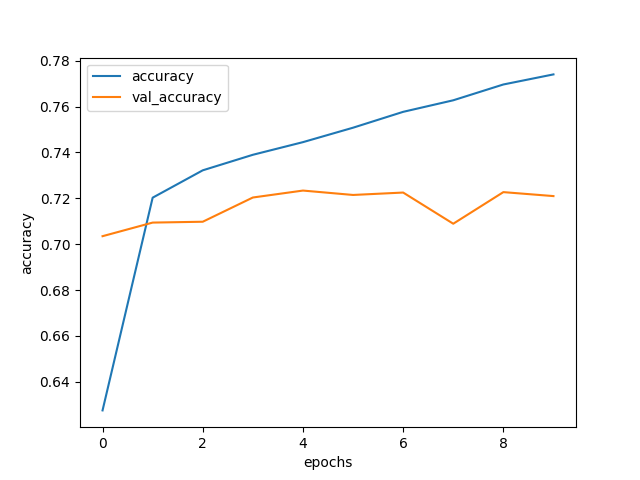
\includegraphics[scale=0.8]{Accuracy_Exp4}
	\caption{Accuracy Graph of Experiment 4}
	\label{fig:accuracy_exp4}
	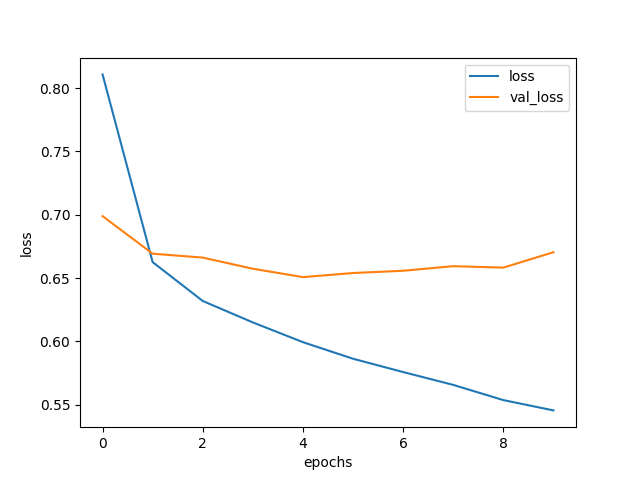
\includegraphics[scale=0.8]{Loss_Exp4}
	\caption{Loss Graph of Experiment 4}
	\label{fig:loss_exp4}
\end{figure}
\pagebreak

\subsection{Experiment 5: Reduced Classification Scope}
\label{exp6}
This is the largest change on an experiment, the ``Neutral'' category has been completely disabled with the purpose of seeing how the rest of the data would be classified as.
\begin{table}[!h]
	\caption{Experiment 5's defining characteristics.}
	\vspace{0.5cm}
	\centering
	\begin{tabular}[t]{|l|l|}
	\hline
		Datasets Used & \makecell{4: \citet{d1}, \citet{d2},\\ \citet{d3}, and \citet{d4}}
	\\ \hline
		Epochs & 10
	\\ \hline
		LSTM Layer & 32 units
	\\ \hline
		Categorized Sentiments as ``Bad'' & ``Sadness'', ``Worry'', and ``Fear''.
	\\ \hline	
		 Categorized Sentiments as ``Neutral'' & N/A
	\\ \hline	
		Categorized Sentiments as ``Good'' & ``Happiness'', ``Fun'', ``Joy'', and ``Love''.
	\\ \hline
	\end{tabular}
\end{table}

\begin{figure}[!h]
	\centering
	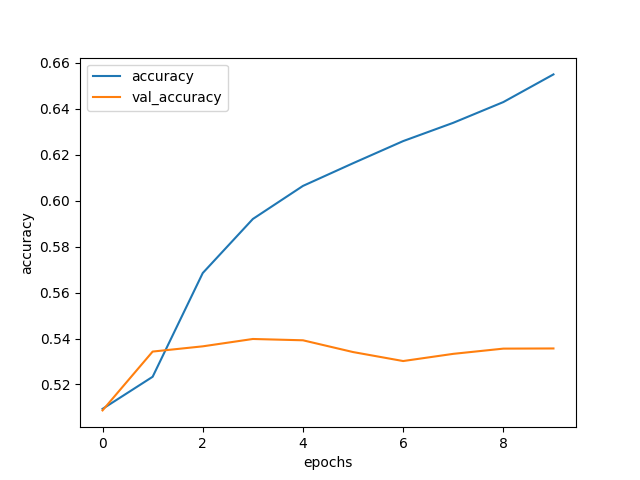
\includegraphics[scale=0.8]{Accuracy_Exp6}
	\caption{Accuracy Graph of Experiment 5}
	\label{fig:accuracy_exp6}
	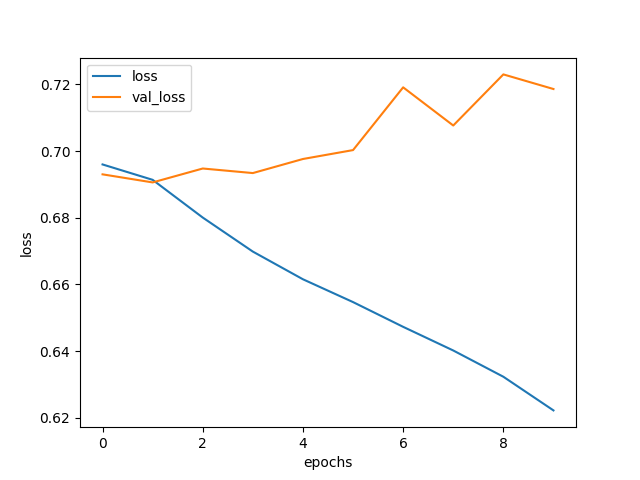
\includegraphics[scale=0.8]{Loss_Exp6}
	\caption{Loss Graph of Experiment 5}
	\label{fig:loss_exp6}
\end{figure}
\pagebreak

\subsection{Experiment 6: Reduced Epochs}
\label{exp7}
Largely the same as previous experiments with half the epochs. This with the purpose of seeing if the data had been overfit.
\begin{table}[!h]
	\caption{Experiment 6's defining characteristics.}
	\vspace{0.5cm}
	\centering
	\begin{tabular}[t]{|l|l|}
	\hline
		Datasets Used & \makecell{4: \citet{d1}, \citet{d2},\\ \citet{d3}, and \citet{d4}}
	\\ \hline
		Epochs & 5
	\\ \hline
		LSTM Layer & 32 units
	\\ \hline
		Categorized Sentiments as ``Bad'' & ``Sadness'', ``Worry'', and ``Fear''.
	\\ \hline	
		 Categorized Sentiments as ``Neutral'' & ``Neutral'' and ``Boredom''.
	\\ \hline	
		Categorized Sentiments as ``Good'' & ``Happiness'', ``Fun'', ``Joy'', and ``Love''.
	\\ \hline
	\end{tabular}
\end{table}


\begin{figure}[!h]
	\centering
	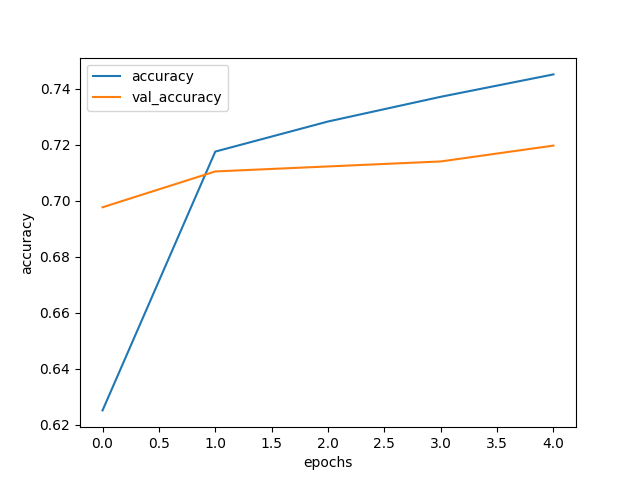
\includegraphics[scale=0.8]{Accuracy_Exp7}
	\caption{Accuracy Graph of Experiment 6}
	\label{fig:accuracy_exp7}
	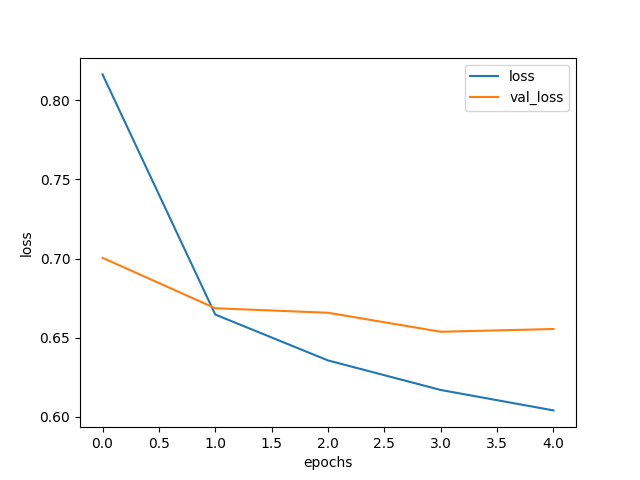
\includegraphics[scale=0.8]{Loss_Exp7}
	\caption{Loss Graph of Experiment 6}
	\label{fig:loss_exp7}
\end{figure}
\pagebreak

\subsection{Experiment 7: Added Stop Words}
\label{exp8}
Same as \nameref{exp7}, the difference being that the top 3 most recurrent words in the datasets are flagged as stop words in an attempt to mitigate the bleed between categories.
\begin{table}[!h]
	\caption{Experiment 7's defining characteristics.}
	\vspace{0.5cm}
	\centering
	\begin{tabular}[t]{|l|l|}
	\hline
		Datasets Used & \makecell{4: \citet{d1}, \citet{d2},\\ \citet{d3}, and \citet{d4}}
	\\ \hline
		Epochs & 5
	\\ \hline
		LSTM Layer & 32 units
	\\ \hline
		Categorized Sentiments as ``Bad'' & ``Sadness'', ``Worry'', and ``Fear''.
	\\ \hline	
		 Categorized Sentiments as ``Neutral'' & ``Neutral'' and ``Boredom''.
	\\ \hline	
		Categorized Sentiments as ``Good'' & ``Happiness'', ``Fun'', ``Joy'', and ``Love''.
	\\ \hline
	\end{tabular}
\end{table}


\begin{figure}[!h]
	\centering
	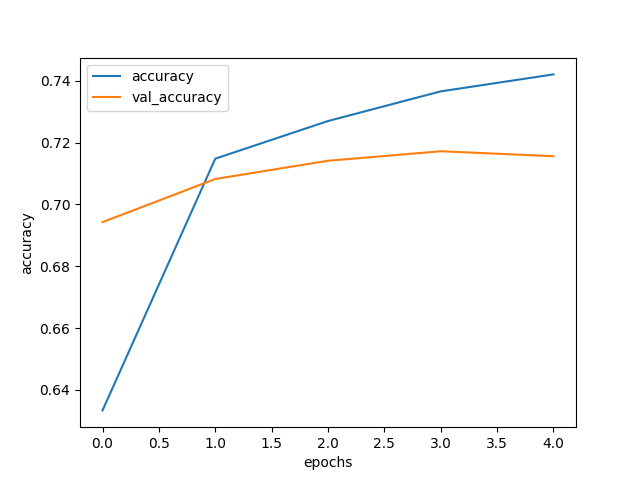
\includegraphics[scale=0.8]{Accuracy_Exp8}
	\caption{Accuracy Graph of Experiment 7}
	\label{fig:accuracy_exp8}
	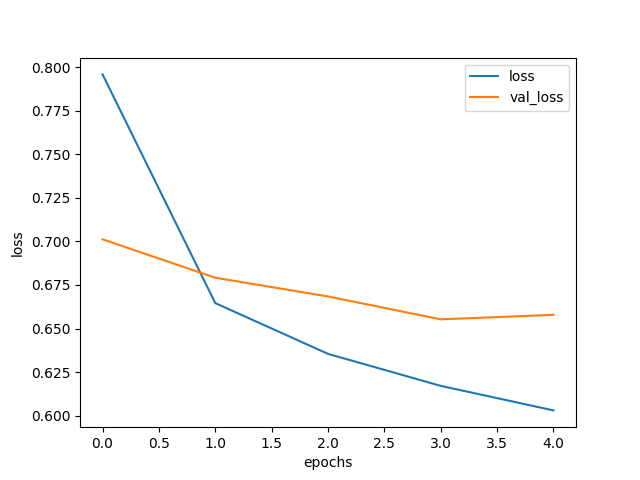
\includegraphics[scale=0.8]{Loss_Exp8}
	\caption{Loss Graph of Experiment 7}
	\label{fig:loss_exp8}
\end{figure}
\pagebreak

\subsection{Experiment 8: Extra Stop Words and Reduced Classification Scope}
\label{exp9}
Keeping in track with \nameref{exp8}, with the added extra of also reducing the scope of the classification, reducing the categories to ``Good'' and ``Bad''.
\begin{table}[!h]
	\caption{Experiment 8's defining characteristics.}
	\vspace{0.5cm}
	\centering
	\begin{tabular}[t]{|l|l|}
	\hline
		Datasets Used & \makecell{4: \citet{d1}, \citet{d2},\\ \citet{d3}, and \citet{d4}}
	\\ \hline
		Epochs & 5
	\\ \hline
		LSTM Layer & 32 units
	\\ \hline
		Categorized Sentiments as ``Bad'' & ``Sadness'', ``Worry'', and ``Fear''.
	\\ \hline	
		Categorized Sentiments as ``Good'' & ``Happiness'', ``Fun'', ``Joy'', and ``Love''.
	\\ \hline
	\end{tabular}
\end{table}


\begin{figure}[!h]
	\centering
	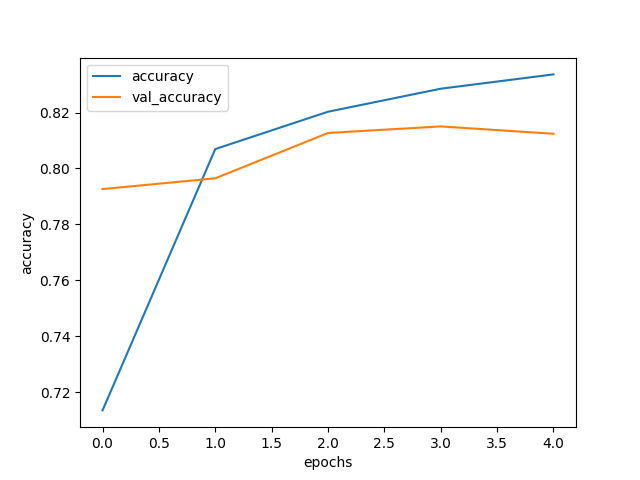
\includegraphics[scale=0.8]{Accuracy_Exp9}
	\caption{Accuracy Graph of Experiment 8}
	\label{fig:accuracy_exp9}
	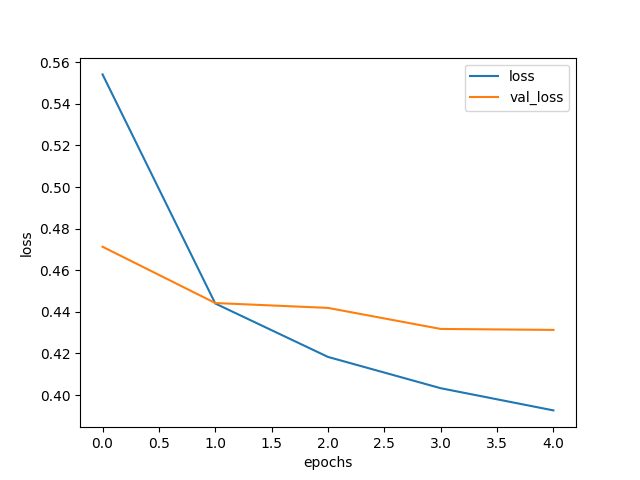
\includegraphics[scale=0.8]{Loss_Exp9}
	\caption{Loss Graph of Experiment 8}
	\label{fig:loss_exp9}
\end{figure}
\pagebreak

\section{Results}
In this section, the results of the experiments from the previous section will be discussed. Later on, a hypothesis will be formulated based from them. For reference, all these experiments were subjected to the same basic test inputs post-training:
\begin{itemize}
	\item ``Good''-labeled sentences: ``I'm happy'' and ``happy happy happy happy happy happy''
	\item ``Neutral''-labeled sentences: ``I don't feel anything'' and an empty input
	\item ``Bad''-labeled sentences: ``I am very sad right now'' and ``sad sad sad sad sad sad sad''
\end{itemize}
\begin{table}[!h]
	\caption{Experimental results}
	\vspace{0.5cm}
	\centering
	\begin{tabular}[t]{|l|l|l|l|l|}
	\hline
	\multicolumn{1}{|c|}{} & \multicolumn{2}{c|}{Training} & \multicolumn{2}{c|}{Cross-Validation}
	\\ \hline
	\ & Loss & Accuracy & Loss & Accuracy
	\\ \hline
	\hyperref[exp1]{Experiment 1} & 0.6916 & 0.7130 & \textbf{0.8709} & 0.6234
	\\ \hline
	\hyperref[exp2]{Experiment 2} & 0.5956 & 0.7576 & 0.7649 & 0.6821
	\\ \hline
	\hyperref[exp3]{Experiment 3} & 0.5829 & 0.7564 & 0.7373 & 0.6780
	\\ \hline
	\hyperref[exp4]{Experiment 4} & 0.5455 & 0.7741 & 0.6704 & 0.7110
	\\ \hline
	\hyperref[exp6]{Experiment 5} & 0.6222 & 0.6550 & 0.7186 & 0.5357
	\\ \hline
	\hyperref[exp7]{Experiment 6} & 0.6041 & 0.7451 & 0.6555 & 0.7097
	\\ \hline
	\hyperref[exp8]{Experiment 7} & 0.6030 & 0.7421 & 0.6579 & 0.7156
	\\ \hline
	\hyperref[exp9]{Experiment 8} & 0.3624 & 0.8337 & 0.3871 & \textbf{0.8124}
	\\ \hline
	\end{tabular}
\end{table}
\pagebreak
\subsection{Interpretation}
In \nameref{exp1}, the post-training results were promising, sentences with obvious ``Good'' and ``Bad'' related words were correctly analyzed. But, as Figures \ref{fig:accuracy_exp1} and \ref{fig:loss_exp1} show, the validation results were considerably worse than the control data scores, this is due to the ``Neutral'' score behaving erratically even when using obvious ``Neutral''-related words, this could be explained by the disparity between words used on the datasets -- not many words were repeated on these --. Even so, overall this had one of the best accuracies across the experiments.

In \nameref{exp2}, using one more dataset and less classes grouped with each category was opted to improve the ``Neutral'' score while trying to keep data across the categories balanced. This had a small impact on the scores but it started to recognize more words as such.

In \nameref{exp3}, seeing that Experiment 2 still struggled to classify ``Neutral'' correctly, more units were given to the LSTM to see if this lowered the chance of error, but as Figures \ref{fig:accuracy_exp3} and \ref{fig:loss_exp3} demonstrate, this got generally the same results. This determined that the defining factor was elsewhere.

In \nameref{exp4}, the base algorithm from Experiment 1 was brought back to work with the three datasets used on Experiments 2 and 3 to verify if the extra dataset was too lopsided to work with. It was found that having the full roster of emotions taken into consideration (``Sadness'', ``Worry'', and ``Fear'', ``Neutral'' and ``Boredom'', ``Happiness'', ``Fun'', ``Joy'', and ``Love'') actually helped the prediction scores. Even so, ``Neutral'' category sentences were still not being recognized correctly sometimes, so more experimentation was needed.

In \nameref{exp6}, some drastic changes were made to experiment with the datasets used, this consisted in completely eliminating the ``Neutral'' category, only taking into consideration ``Bad'', ``Good'' and ``0'' with the intention of seeing the algorithm's behavior. This worked. 

In \nameref{exp7}, taking again into consideration the results given from Experiment 5, the problem of overfitting was also a concern, and since the epoch count was a parameter yet-to-be manipulated. Instead of using the usual 10 epochs, 5 were used. This did not have any noticeable effect in the prediction output, however.

In \nameref{exp8}, manually marking the words that represent the most bleed between categories (``work'', ``go'', ``nt'') still wasn't enough to fix the categorization problem, even though there was a slight benefit in the accuracy and loss values.

In \nameref{exp9}, reducing the data category scope while also maintaining the stopwords mentioned on Experiment 7 filtered, brought overall the best results as of yet. This can be attributed to the fact that the most significant category bleed happened between ``Neutral'' and ``Bad'' since they shared a lot of the word pool.

\subsection{Discussion}
The experiment with the best performance overall was \nameref{exp9}, with the scope adjustment the goal of predicting, at least partially, the feeling of a person's input was achieved. Thanks to an exhaustive search conducted inside all of the datasets used it was found out that the most-used words in the datasets pertaining to the ``Bad'' and ``Neutral'' category were mostly ambiguous words that, out of context, could be interpreted as disinterest or overall any other emotion.
\begin{figure}[!h]
	\centering
	\includegraphics[scale=0.7]{word clouds old/neutral_words.png}
	\caption[Word cloud of the ``Neutral'' category's corpus previous to the filtering.]{Word cloud of the ``Neutral'' category's corpus previous to the filtering in \nameref{exp8}}
	\label{fig:neutralwords_pre}
	\vspace{1cm}
	\includegraphics[scale=0.7]{word clouds old/sadness_words.png}
	\caption[Word cloud of the ``Bad'' category's corpus previous to the filtering]{Word cloud of the ``Bad'' category's corpus previous to the filtering in \nameref{exp8}}
	\label{fig:sadnesswords_pre}
\end{figure}

This, combined with the fact that some of the datasets used were plagued with orthographical errors, affected the performance of this algorithm's original scope. Thus, \hyperref[exp9]{Experiment 8} had to reduce the scope.

\begin{figure}[!h]
	\centering
	\includegraphics[scale=0.7]{word clouds new/neutral_words.png}
	\caption{Word cloud of the ``Neutral'' category's corpus post-filtering}
	\label{fig:neutralwords_post}
	\vspace{1cm}
	\includegraphics[scale=0.7]{word clouds new/sadness_words.png}
	\caption{Word cloud of the ``Bad'' category's corpus post-filtering}
	\label{fig:sadnesswords_post}
\end{figure}

These results determine that the proposed hypothesis is partially true: given enough data, a Machine Learning algorithm can learn to classify feelings and react accordingly, effectively learning how to identify patterns to an extent. However, high quality and volume data is needed for this to be reliable. Something that was only partially obtained for this project.

Overall, we can determine that, with the use of more consistent data, a favorable result can be achieved with the model used in this project.

\appendix
%%% Haz un documento para cada apéndice
%%%\\chapter{Este es un apéndice}

\section{Citas bibliográficas}

\section{Comillas}



\backmatter
\pagestyle{main}

%%% Aquí va la bibliografía, puedes usar el entorno de LaTeX (thebibliography)
%%% o la herramienta BibTeX. En caso de que optes por BibTeX, puedes usar
%%% alguno de los archivos de estilo (mighelbib.bst o mighelnat.bst) incluidos
%%% en el paquete, cuyos diseños armonizan con el diseño de tesis provisto por
%%% fime.cls. Para muestra, basta un botón:

\bibliographystyle{plainnat}
\bibliography{biblio}

\label{lastpage}
%Autobiografia

\chapter*{Resumen autobiográfico}
\thispagestyle{empty}

\begin{center}
\autor

Candidato para obtener el grado de\\
\grado\\
\orientacion\bigskip

\uanl\\
\fime\bigskip

Tesis:\\
\textsc{\large\titulo}
\end{center}\bigskip

%Aquí va tu historia
Aquí va tu historia. Recuerda que debe incluir: lugar y fecha de nacimiento, nombre de los padres, escuelas y universidades en las que se graduó después de la preparatoria, títulos o grados obtenidos (no incluir los estudios que se están concluyendo), experiencia profesional y organizaciones profesionales a las que pertenece (no incluir lista de publicaciones).


\end{document}
